
\chapter{Uma revolução}

\section{O rei do rock'n roll}

% Exemplo de imagem.
\begin{figure}[!htb]
  \centering
  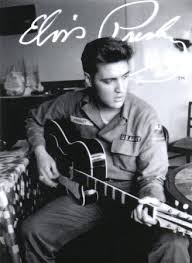
\includegraphics[scale=0.45]{imagens/elvis}
  \caption{Elvis Presley no início de sua carreira.}
  \label{fig:elvis}
\end{figure}

Um dos artistas mais importantes dos primeiros anos do {\it rock’n’roll} foi Elvis Presley. Como explica 
Chacon \cite{CHA1985}, ``só um símbolo sexual, devidamente municiado pelos melhores autores e ‘cantando e 
suando 
como um 
negro`` poderia transformar aquele modismo numa verdadeira revolução”. A sensualidade presente na voz rouca 
e 
na sua maneira de dançar, que transformaram Elvis numa superestrela do rock, tornou-o um exemplo clássico da 
influência negra sobre a sociedade branca norte-americana \cite{CHA1985}. Além disso, sua história também 
tem pontos em comum com a de outros artistas: vidas atribuladas, 
envolvimento com drogas, relacionamentos desfeitos e um triste fim. Estes foram também alguns dos 
ingredientes das vidas de Jerry Lee Lewis, que teve muitos problemas com bebida e se casou várias vezes ou 
de Buddy Holly, que morreu ainda jovem em um desastre de avião.
  
\section{A Era Beatles}

No início de 1956, John Lennon formou o conjunto {\it The Quarrymen}, que nada mais era do que uma reunião 
informal 
de amigos. O grupo se estabilizaria em 1960, com Paul McCartney e George Harrison como guitarristas, Stu 
Sutcliffe no baixo e o baterista Pete Best.

Neste mesmo ano, The Quarrymen deixa de existir; em seu lugar, surge uma “banda profissional de 
{\it rock’n’roll}, os Beatles. O nome foi uma combinação da palavra beetle (besouro) com uma expressão 
comum à 
época para o rock: música {\it beat}. A referência aos insetos foi uma homenagem ao grupo de Buddy Holly, 
chamado 
{\it Crickets} (grilos).

Em 1962, os Beatles foram tocar em Hamburgo, Alemanha, quando encontraram o baterista Ringo Starr, que 
tocava com os {\it Hurricanes}. Pouco tempo depois, ele substituiria Pete Best.

\subsection{A explosão dos Beatles}

Finalmente em agosto deste mesmo ano, o grupo entraria nos estúdios de {\it Abbey Road} para a gravação 
do 
primeiro compacto da banda, com as músicas {\it P.S. I Love You} e {\it Love me Do}. Nesta época, Stu 
Sutcliffe havia 
deixado os {\it Beatles} e Paul tomou a posição de baixista do grupo.
Com o segundo single, {\it Please Please Me}, os {\it Beatles} alcançaram o topo das paradas britânicas.

Em 1963, apenas um ano depois do primeiro lançamento dos {\it Beatles}, a {\it Beatlemania} eclodiu na 
Inglaterra. 
Brian Epstein e o produtor George Martin, da EMI, decidem partir com a banda para os Estados Unidos, cientes 
da popularidade do grupo. Em 1964, os Beatles conquistam a América com {\it I Want to Hold Your Hand}. A 
apresentação da banda no programa de televisão de Ed Sullivan – o mesmo que tinha lançado Elvis Presley – 
foi a alavanca para que a mídia norte-americana passasse a publicar matérias sobre os {\it Fab Four} (como 
eram 
conhecidos).

\begin{figure}[!htb]
%  \vspace{1cm}
  \centering
  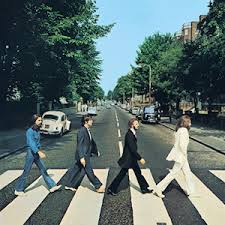
\includegraphics[width=7cm]{imagens/abbey_road}
  \caption{Capa do Album Abbey Road, de 1969.}
  \label{fig:abbeyroad}
%  \vspace{1cm}
\end{figure}

Durante os shows dos {\it Beatles}, quase não se ouvia suas músicas, devido à 
quantidade 
de garotas que gritavam 
histericamente pelos músicos. A partir de 1965, o grupo passou a se preocupar mais com as composições, 
deixando o amor romântico de lado e empenhando-se em explorar outros temas. O disco {\it Rubber Soul}, 
lançado 
neste mesmo ano, marca o amadurecimento da banda, visível na crítica social da música {\it Nowhere Man} ou 
nas 
referências abstratas de {\it Norwegian Wood}, entre outras composições deste disco.


\section{Pedras que rolam}

Entretanto, não só do sucesso dos {\it Beatles} vivia a Inglaterra. {\it Rolling Stones} e {\it The Who} 
são exemplos de 
grupos que surgiram na década de 60 e que marcaram o rock em muitos sentidos.

O verso de uma canção de blues de Muddy Waters – {\it rolling stones gather no moss} (pedras que rolam não 
criam 
musgo) - dá o nome ao conjunto fundado pelo guitarrista Brian Jones. O vocalista, Mick Jagger, torna-se o 
líder da banda após a saída de Jones. A influência negra é uma das marcas do grupo, além da sensualidade e 
uma certa androginia, características da performance de Jagger.

Em 1968, os {\it Stones} exploram o engajamento político na música {\it Street Fighting Man}, influenciados 
pelas 
manifestações políticas de massa que emergiam. A música, composta por Mick Jagger e Keith Richards, torna-se 
hino dos revolucionários e é censurada pela polícia de Chicago.

A música dos {\it Stones} é da mesma época de {\it Revolution}, dos {\it Beatles}. Esta última também foi 
composta a partir do 
contexto político-social de 1968, marcado principalmente pelas manifestações de maio deste mesmo ano. Os 
críticos passam a analisar {\it Revolution} e {\it Street Fighting Man} e a compará-las, sendo que 
consideram a primeira 
como uma “contra-revolução” e a segunda como a “verdadeira revolução”. Mas, tanto as últimas estrofes da 
música dos Stones quanto uma declaração de Jagger – “Eles devem pensar que ‘{\it Street Fighting Man}’ é 
capaz de 
promover uma revolução\ldots Eu bem que gostaria que isso fosse verdade” – demonstram que a idéia dos 
críticos se baseia em suposições.

\section{Melhores riffs da história do rock}

De acordo com a revista The Sun, estes são os 5 melhores riffs da história do rock.

% Exemplo de tabela
\begin{table}[!htb]
  \centering
  \caption{Melhores riffs da história do rock, de acordo com a revista The Sun.}
  \vspace{0.1cm}
\begin{tabular}{|c|c|c|}
\hline
\textbf{Posição} & \textbf{Nome da Música} & \textbf {Nome da banda} \\
\hline
1 & Sweet Child O'Mine & Guns 'N Roses  \\
\hline
2 & Layla & Eric Clapton \\
\hline
3 & Walk This Way & Aerosmith \\
\hline
4 & Beat It & Michael Jackson \\
\hline
5 & Ace of Spades & Motörhead \\
\hline
% 6 & Voodoo Child & Jimi Hendrix \\
% \hline
% 7 & Another One Bites the Dust & Queen \\
% \hline
% 8 & Smell Like Teen Spirit & Nirvana \\
% \hline
% 9 & Smoke on the Water & Deep Purple \\
% \hline
% 10 & American Idiot & Green Day \\
% \hline
\end{tabular}

\end{table}